% Start preamble
\documentclass[12pt,a4paper]{article}
\usepackage{geometry}
 \geometry{
 a4paper,
 total={170mm,257mm},
 left=20mm,
 top=20mm,
 }
\usepackage[utf8]{inputenc}
\usepackage[T1]{fontenc}
\usepackage[pdftex]{graphicx}
\graphicspath{{./}}
\usepackage{enumitem}
\usepackage{pdfpages}
\usepackage{hyperref}
\usepackage{tikz}
\usepackage{attachfile}
\usepackage{epstopdf}
\usepackage{array}
\usepackage{multirow}
\usepackage{multicol}
\usepackage{float}
%\usepackage[table]{xcolor,colorbl}
\setlength{\textwidth}{16cm}
\setlength{\oddsidemargin}{-0.5cm}
\setlength{\evensidemargin}{-0.5cm}
%\setlenght{\headsep}{0cm}
\setlength\parindent{0pt}
%\setlength{\extrarowheight}{3pt}
\usepackage{listings}
%\usepackage{xcolor}
\definecolor{mGreen}{rgb}{0,0.6,0}
\definecolor{mGray}{rgb}{0.5,0.5,0.5}
\definecolor{mPurple}{rgb}{0.58,0,0.82}
\definecolor{backgroundColour}{rgb}{0.95,0.95,0.92}

\lstdefinestyle{CStyle}{
backgroundcolor=\color{backgroundColour},   
commentstyle=\color{mGreen},
keywordstyle=\color{magenta},
numberstyle=\tiny\color{mGray},
stringstyle=\color{mPurple},
basicstyle=\footnotesize,
breakatwhitespace=false,         
breaklines=true,                 
captionpos=b,                    
keepspaces=true,                 
numbers=left,                    
numbersep=5pt,                  
showspaces=false,                
showstringspaces=false,
showtabs=false,                  
tabsize=2,
language=C
 }
\input{arduinoLanguage.tex}
%%%%%% Counting oppgaves %%%%%%
 \newcount\questnum \questnum=0
 \def\oppgave{
            \advance\questnum by 1
	    \ifthenelse{\questnum>0\AND \questnum<9}
	    {
                \vskip 1cm
		\textbf{Oppgave}\hskip 5pt\the\questnum \hfill \hfill(6p)
		\vskip 3pt
		\hrule
	\vskip 0.5cm}
	{
                \vskip 1cm
		\textbf{Oppgave}\hskip 5pt \the\questnum \hfill \hfill(12p)
		\vskip 3pt \hrule \vskip 0.5cm }

		}
 %%%%%%%%%%%%%%%%%%%%%%
%%%%%%%%%%%%%%%%%%%%%%


% End preamble

\begin{document}
% !TEX root = /home/fred-olav/afgv/src/preamble.tex
\LARGE
\centerline{\bf Prøve i måleteknikk 21/22}  \bigskip
\normalsize
Følgende kompetansemål er relevante for prøven:
\begin{itemize}[noitemsep]

	\item planlegge, utføre, vurdere kvalitet, sluttkontrollere og dokumentere arbeidet
	\item montere, konfigurere, kalibrere og idriftsettelse digitale og analoge målesystemer
\end{itemize}



Mål som eleven prøves i på prøven: 
\begin{itemize}[noitemsep]
\item Kjenne til, forklare og regne på grunnleggende fysikk for målemetodene.
% trykk, 
\item Kunne forklare virkemåten til måleprisnippene og ferdige målesystemer. 
\item Kunne kalibrere instrumentene
\item Kunne planlegge og beskrive montering og dokumentasjon av et målesystem. 
\item Kunne grunnleggende prinsipper fra tidligere emner. 
\end{itemize}



Oppgave 1-8 gjøres med håndbok og skal leveres på papir. \\
Oppgave 9 skal gjøres i på PC og føres i et word  dokument og sendes på mail til fred-olav.mosdal@skole.rogfk.no\\

\bigskip 
\hrule
\bigskip 
\textbf{Navn:}\bigskip 
\hrule
\vfil \eject

\oppgave{} 
\vskip 5pt
% Elektroteknikk
Regn ut resistansen til strekklappen i denne målebro kretsen, gitt voltmeterets indikasjon på 1.76228mV (A er positiv og B er negativ).

$$\includegraphics[width=15.5cm]{i04867x01.eps}$$

Gitt at dette er et PT100 element fra europa, hvilken temperatur måler elementet?

\vskip 1cm 

\begin{tikzpicture}
	\draw[step=0.5cm,gray!40,very thin]  grid (16,12) ;
\end{tikzpicture}

\newpage
\oppgave{} 
Beskriv følgende faguttrykk brukes til:
\begin{itemize}[noitemsep]
	\item termolomme
\end{itemize}

\begin{tikzpicture}
	\draw[step=0.5cm,gray!40,very thin]  grid (16,3.5) ;
\end{tikzpicture}
\begin{itemize}[noitemsep]
	\item impulsrør
\end{itemize}

\begin{tikzpicture}
	\draw[step=0.5cm,gray!40,very thin]  grid (16,3.5) ;
\end{tikzpicture}
\begin{itemize}[noitemsep]
	\item bleed fittings
\end{itemize}

\begin{tikzpicture}
	\draw[step=0.5cm,gray!40,very thin]  grid (16,3.5) ;
\end{tikzpicture}
\begin{itemize}[noitemsep]
	\item kompensajonskabel
\end{itemize}

\begin{tikzpicture}
	\draw[step=0.5cm,gray!40,very thin]  grid (16,3.5) ;
\end{tikzpicture}
\begin{itemize}[noitemsep]
	\item strømningsretter
\end{itemize}

\begin{tikzpicture}
	\draw[step=0.5cm,gray!40,very thin]  grid (16,3.5) ;
\end{tikzpicture}
\begin{itemize}[noitemsep]
	\item måleblende
\end{itemize}

\begin{tikzpicture}
	\draw[step=0.5cm,gray!40,very thin]  grid (16,3.5) ;
\end{tikzpicture}


\oppgave{} 
Lagringstanken nedenfor inneholder heptan med en $\rho=684kg/m³$. En DP-celle i bunn av tanken måler nivået ved hjelp av det hydrostatikse trykket av heptanen. %The following storage vessel holds liquid heptane, a hydrocarbon with an approximate specific gravity of 0.68.  A pressure transmitter located at the bottom infers heptane level by hydrostatic pressure (head).  Determine the calibration range of this pressure transmitter in order to properly translate the range of vessel level (0 to 14 feet) into an output signal of 4 to 20 mA.  Please express the transmitter's calibration range in units of inches W.C. (inches of water column).

$$\includegraphics[width=15.5cm]{i00241x01.eps}$$

Finn ut følgende: 

\begin{itemize}
	\item  måleområde denne DP-cellen må ha for å kunne igjengi nivået i tanken fra 0-4.5m, som et utgangssignal på 4-20mA. 
	\item{} Utgangsignalet fra DP-cellen ved et nivå på 1.5m 
	\item{} Nivået med Heptan ved et utgangssignal på 5.7mA.
\end{itemize}

\begin{tikzpicture}
	\draw[step=0.5cm,gray!40,very thin]  grid (16,25) ;
\end{tikzpicture}
\newpage
\oppgave{} 
\vskip 2.5pt 
a) Konverter en volumetrisk strømningsrate på 345 l/m kvikksølv ($\rho=13546 kg/m^3$ om til en masse strøm oppgitt i kg/h
\vskip 2.5pt 

\begin{tikzpicture}
	\draw[step=0.5cm,gray!40,very thin]  grid (16,4) ;
\end{tikzpicture}
\vskip 0.5cm 
b) Vi har et rør som det strømmer olje med en strømningsrate på 200 m³/h og en temperatur på 50°C. Begge seksjonene er etter schedule 40.  Den første delen av røret har dimensjon DN200 (ID=202.74mm) og den andre delen har dimensjon DN65 (ID=62.68mm)
$$\includegraphics[width=15.5cm]{aFlow01x02.eps}$$
Regn ut hastigheten til fluidet i hver av seksjonene. 
\vskip 2.5pt 

\begin{tikzpicture}
	\draw[step=0.5cm,gray!40,very thin]  grid (16,8) ;
\end{tikzpicture}
\newpage
\oppgave{} 
Vis hvordan dette målesystemet med et PT100 element må kobles for at displayet skal vise temperaturen. Sørg for å gjøre en  oppkobling som kanselerer effekten av leder resistant fult ut. 

$$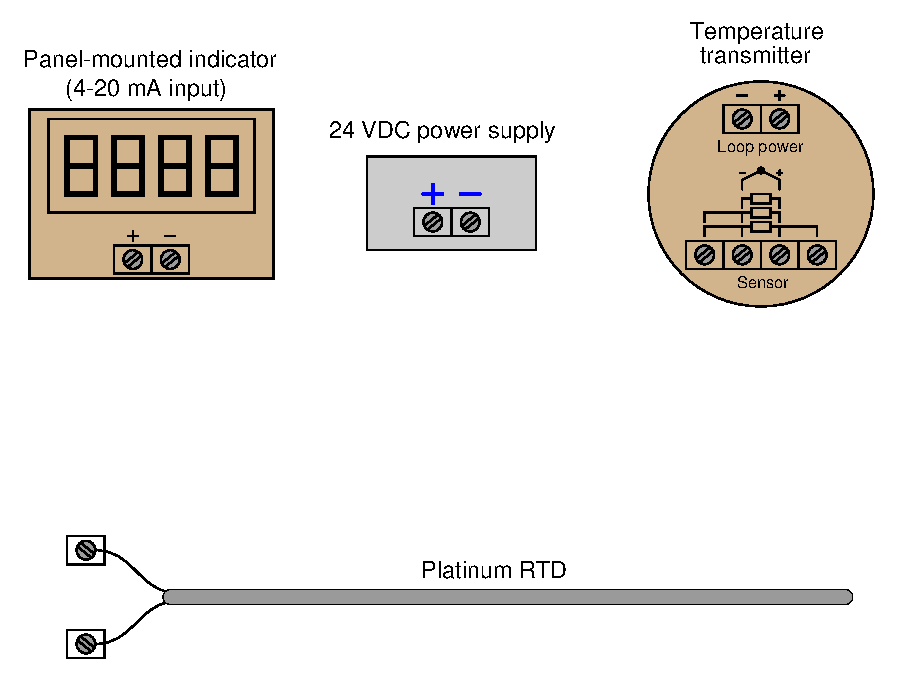
\includegraphics[width=15.5cm]{i04000x01.eps}$$

\begin{tikzpicture}
	\draw[step=0.5cm,gray!40,very thin]  grid (16,6) ;
\end{tikzpicture}
\newpage
\oppgave{} 
Tegn og forklar virkemåten til en ultralyd nivåmåler

\vskip 0.5cm

\begin{tikzpicture}
	\draw[step=0.5cm,gray!40,very thin]  grid (16,23) ;
\end{tikzpicture}
\newpage
\oppgave{} 
Tegn og forklar virkemåten til en DP-celle med kapasitivt måleelement. `
\vskip 0.5cm

\begin{tikzpicture}
	\draw[step=0.5cm,gray!40,very thin]  grid (16,23) ;
\end{tikzpicture}
\newpage
\oppgave{} 
Tegn og forklar virkemåten til et målesystem for stømning basert på måleblende. 
\vskip 0.5cm

\begin{tikzpicture}
	\draw[step=0.5cm,gray!40,very thin]  grid (16,23) ;
\end{tikzpicture}
\newpage
\oppgave{} 
Du har fått i oppgave å montere og koble til en elektromagnetisk flowmåler i et vannforsyningsanalegg. Rørdimensjonen der måleren skal monteres er DN300(12 tommer). Røret er i metall. Klargjøring av flenser på røret gjøres av en mekanikker i firmaet. 
\vskip 1cm 
Vis hvordan du ville planlagt, gjennomført og dokumentert jobben

\vskip 1cm 

Oppgave 9 leveres i en PDF fil som sendes på mail til:
\vskip 1cm 
fred-olav.mosdal@skole.rogfk.no\\
Emnefeltet skal bestå av følgende:
Måleteknikk
\end{document}
